	La parte central del presente trabajo está constituida por el módulo de interfaz entre el FPGA y la PC, que es el que permite cumplir el objetivo de proveerle al sistema la comunicación, es decir, que cualquier dispositivo implementado con FPGA pueda recibir y transmitir datos a través del protocolo USB desde y hacia una PC, respectivamente.%\\
	
	La interfaz está constituida por el controlador EZ-USB FX2LP fabricado por Cypress Semiconductor, un circuito integrado que posee en su interior un microcontrolador 8051, con algunas mejoras destinadas a satisfacer mejor los requerimientos del sistema USB; una interfaz serie, que permite ingresar datos uno tras otro y los entrega en forma paralela y viceversa; un transceptor USB encargado de todas las tareas de codificación y decodificación de paquetes USB; memoria RAM para programas y datos de \SI{16}{\kilo\byte}. Posee, a su vez, tres tipos de interfaces hacia periféricos externos: I$^2$C, una memoria FIFO (Primero Entrado, Primero Salido, del inglés{\it First In First Out}) destinada a sistemas con poder de iniciativa para escribir y leer datos, y un sistema de propósito general que puede ser comandado a través del 8051\cite{CypressSemiconductor2014fx2lp}.%\\%a través del cual efectua las tareas que requiere la comunicación USB, sumado a un transceptor USB, el cual codifica y decodifica los paquetes USB que se transmiten a través del bus. A su vez, posee ciertos periféricos e interfaces que otorgan flexibilidad suficiente para adecuar el chip a los requerimientos de un desarrollo determinado.\\
	
	El controlador viene montado en un circuito impreso que posee una serie de componentes adicionales que facilitan la interacción del desarrollador, tales como pulsadores, display de 7 segmentos, módulos de memoria adicional,etc. Este tipo de circuitos impresos armados con la intención de favorecer desarrollo de otros sistemas, se denomina placa de desarrollo. Una placa de desarrollo que, además, incorpora algunas herramientas extra como software, cables de conexión, fuentes, etc. toma el nombre de kit de desarrollo.%\\

	\begin{figure}
	\centering
	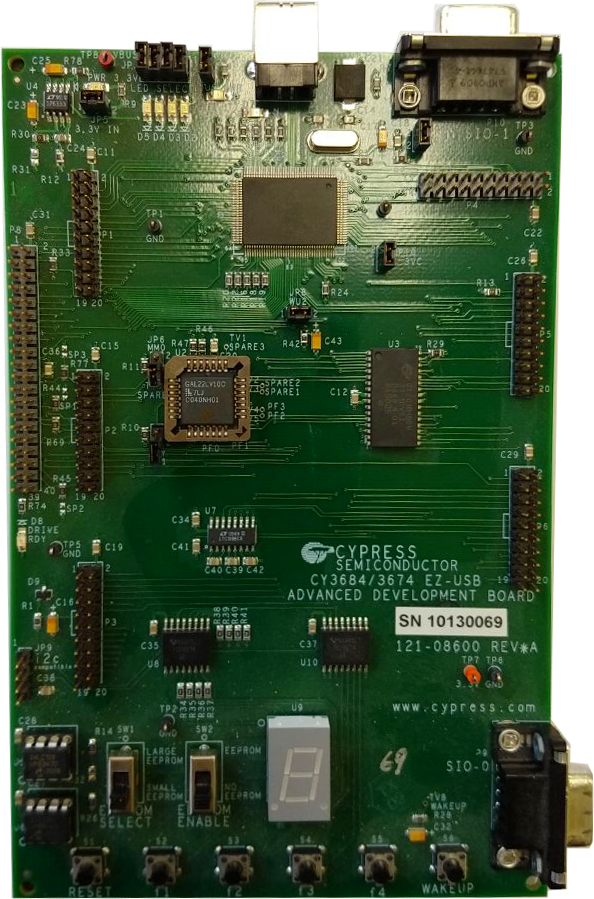
\includegraphics[width=0.4\textwidth]{32cypressboard}
	\caption{Circuito impreso principal del kit de desarrollo CY3684 EZ-USB FX2LP}
	\label{fig:cy3684}
	\end{figure}
	
	En este trabajo, se utiliza el kit de desarrollo CY 3684 EZ-USB FX2LP, fabricado por Cypress Semiconductor\cite{CypressSemiconductor2014cy3684}. El kit posee una placa de desarrollo como la que se observa en la Figura \ref{fig:cy3684}. El componente principal del kit es el controlador EZ-USB FX2LP e incorpora un display de 7 segmentos, 4 luces led multipropósito, 6 pulsadores, de los cuales 4 son de propósito general, uno de reinicio y otro que envía una señal especial para salir de un modo de bajo consumo. También tiene dos bloques de memorias EEPROM destinadas al almacenamiento del firmware (programa que ejecuta un microcontrolador), lo que otorga la posibilidad de realizar una carga no volátil de la configuración del controlador, memoria flash de \SI{64}{\kilo\byte} utilizados como RAM por el programa del controlador, un puerto USB y dos puertos UART con zócalos DE-9. Adicionalmente, cuenta con 6 puertos de 20 pines que permiten comunicarse con el controlador y 1 puerto de 40 pines, compatible con el protocolo ATA.%\\
	%AQUI QUEDE
	
%	La arquitectura del controlador EZ-USB FX2LP se muestra en la Figura %TODO la arquitectura, pavo
%	. En ella se puede apreciar los diferentes componentes que se integran en él. Como se menciona anteriormente, la serie de circuitos integrados EZ-USB FX2LP incorporan un microcontrolador 8051, con algunas mejoras destinadas a satisfacer mejor los requerimientos del sistema USB; una interfaz serie, que permite ingresar datos uno tras otro y los entrega en forma paralela y viceversa; un transceptor USB encargado de todas las tareas de codificación y decodificación de paquetes USB; memoria RAM para programas y datos de \SI{16}{\kilo\byte}. Posee, a su vez, tres tipos de interfaces hacia periféricos externos
	 
	
%	Como interfaz entre la FPGA y la PC se utilizó kit de de desarrollo CY3684 FX2LP EZ-USB Development Kit de Cypress Semiconductor,la que se observa en la Figura \ref{cy3684}. Esta placa posee como núcleo el controlador USB CY7C68013A, circuito integrado que posee todas las herramientas necesarias para realizar la interfaz, como así también un buen número de periféricos que permiten al desarrollador realizar pruebas y depuración.\\
	
	
%	Entre estas, se destacan 6 pulsadores, de los cuales cuatro se utilizan para proposito general, uno para reestablecer los valores por defecto de la placa y uno para enviar señales de suspensión y reestablecimiento del programa actualmente cargado en el microcontrolador, lo que coloca al sistema en modo bajo consumo de energía. A su vez, posee dos memorias EEPROM que sirven para cargar firmware y archivos de configuración del sistema, un display de 8 segmentos, 4 leds de multiple propósito, dos puertos UART, una salida de pines compatible con puertos ATA y 6 puertos de 20 pines que se utilizan para la conexión hacia el chip núcleo. Como soporte para el firmware, posee también un bloque con \SI{64}{\kilo\byte} de memoria SRAM.\\
	
	Se selecciona este controlador como interfaz ya que cuenta con una gran cantidad de herramientas que permiten realizar la comunicación USB, además de poseer memoria suficiente para datos y una interfaz de comunicación para periféricos simple lo que facilita el objetivo de utilizar la menor cantidad de los recursos configurables del FPGA, de forma tal que queden, estos últimos, disponibles para el desarrollo de otros sistemas.%\\
	